\section{Công trình liên quan}

\begin{frame}{Các phương pháp}
		
	\textbf{Rule Base \& Statistic}
	\begin{itemize}
		\small
		\item BEAT, Rule-based generation.
		%					 \cite{cassell2001beat}
		\item Gesture Controllers 
	\end{itemize}
	%	\textit{Nhược điểm}: Không có khả năng mở rộng, kết quả không tốt với các dữ liệu ngoài tập huấn luyện.
	\textbf{Phase Manifold} : 
	
	\begin{itemize}
		\small
		\item  DeepPhase , Walk the Dog
	\end{itemize}
	
	\textbf{Deep Learning}
	\begin{itemize}
		\small
		\item \textbf{MLP}: Gesticulator
		\item \textbf{RNN}: Speech2AffectiveGestures, HA2G, TransGesture, .. 
		\item \textbf{Normalising Flows}: Text2gestures, Speech2Gesture,; \textbf{GAN}: DiffGAN
		\item \textbf{VAE/VQ-VAE}:  Audio2Gestures; 
		\item \textbf{Diffusion}: Listen denoise action, DiffuseStyleGesture, Taming Diffusion Models.
		
	\end{itemize}

\textbf{Baseline}: \textit{Motion Diffusion Model} (MDM)

%\begin{columns}
%\begin{column}{0.55\textwidth}
	
%\end{column}			
% 
%	
%	\begin{column}{0.45\textwidth}
%		
%		\begin{columns}
%			\begin{column}{0.5\textwidth}
%				\begin{figure}
%					\includegraphics[width=\textwidth]{ProbabilityDensityFunctions.png}
%					\caption{\scriptsize Phải chuẩn hoá (diện tích dưới đường cong phải tích phân thành một)}
%				\end{figure}
%			\end{column}
%			\begin{column}{0.5\textwidth}
%				\begin{figure}
%					\includegraphics[width=\textwidth]{ScoreFunction.png}
%					\caption{\scriptsize Không cần chuẩn hoá.}
%				\end{figure}
%			\end{column}
%		\end{columns}
%		
%
%		
%		\begin{columns}
%			\begin{column}{0.5\textwidth}
%				\centering
%				\begin{tikzpicture}
%					\node at (0, 1) {$p(\mathbf{x})$};
%					
%					\node at (0, 0.5) {\small \text{probability density}};
%					
%					\draw[<->, thick] (0, 0) -- (0, -0.5);
%					
%					\node at (0, -1) {$\nabla_\mathbf{x} \log p(\mathbf{x})$};
%					
%					\node at (0, -1.5) {\small \text{score function}};
%				\end{tikzpicture}
%				
%			\end{column}
%			\begin{column}{0.5\textwidth}
%				\begin{figure}
%					\includegraphics[width=\textwidth]{CompareScoreFunction.png}
%					\caption{\scriptsize score function vs probability density}
%				\end{figure}
%			\end{column}
%		\end{columns}
%	\end{column}
%\end{columns}

%\includegraphics[width=\linewidth]{../animation/ScoreFunction/ScoreFunction\_001}
	
\end{frame}


\begin{frame}{Overview Diffusion Model}
%\begin{columns}
%	\begin{column}[T]{0.5\textwidth}
%	
%		
%	\end{column}
%	
%	\hspace*{-1em}
%	
%	\begin{column}[T]{0.5\textwidth}
%		
%	\end{column}
%\end{columns}

\textbf{Forward Diffusion Process (Fixed)}
\begin{equation}
	\mathbf{x}_t=\sqrt{1- \beta_t} \cdot \mathbf{x}_{t-1}+\sqrt{\beta_t} \cdot \epsilon
\end{equation}

hay $\mathbf{x}_{t-1} = \frac{1}{\sqrt{1-\beta_{t}}} (\mathbf{x}_t - \sqrt{\beta_t} \cdot \epsilon) $

%	\[
%	q(x_t | x_{t-1}) = \mathcal{N}(x_t; \sqrt{1 - \beta_t} \, x_{t-1}, \beta_t \, I)
%	\]

%	Ta gọi $\epsilon = \mathcal{N}(0, I)$
\begin{columns}
\begin{column}{0.8\textwidth}
\begin{figure}
	\centering
	\includegraphics[width=\textwidth]{OverviewDiffusion}
\end{figure}
\end{column}

\begin{column}{0.2\textwidth}
\includegraphics[width=\textwidth]{SquareBeta}
\end{column}
\end{columns}


\textbf{Reverse Diffusion Process}

\begin{equation}
	\mathbf{x}_{t-1}=\frac{1}{\sqrt{1- \beta_t}}\left(\mathbf{x}_t-\sqrt{\beta_t} \cdot \epsilon_{\color{red}{\theta}}\left(\mathbf{x}_t, t\right)\right)+\color{red}{\beta_t \cdot \sigma_t \mathbf{z}} \color{black}{}
\end{equation}
%\mathcal{N}(0, I)

\end{frame}
	
\begin{frame}{Forward Diffusion Process}
%	 & \text{ ;where } \boldsymbol{\epsilon}_{t-1}, \boldsymbol{\epsilon}_{t-2}, \dots \sim \mathcal{N}(\mathbf{0}, \mathbf{I})
\small
\begin{itemize}[]
	\item Đặt $\alpha_t = 1 - \beta_t$, $\bar{\alpha}_t = \prod_{i=1}^t \alpha_i$
\end{itemize}
\vspace{-15pt}
\begin{align*}
	\mathbf{x}_t & = \sqrt{\alpha_t}\mathbf{x}_{t-1} + \sqrt{1 - \alpha_t} \boldsymbol{\epsilon}_{t-1} \\
						& = \sqrt{\alpha_t \alpha_{t-1}} \mathbf{x}_{t-2} + \sqrt{1 - \alpha_t \alpha_{t-1}} \bar{\boldsymbol{\epsilon}}_{t-2} \\
						& = \dots \\
						& = \sqrt{\bar{\alpha}_t}\mathbf{x}_0 + \sqrt{1 - \bar{\alpha}_t}\boldsymbol{\epsilon} \\
						q(\mathbf{x}_t \vert \mathbf{x}_{t-1}) &= \mathcal{N}(\mathbf{x}_t; \sqrt{\alpha_t} \mathbf{x}_{t-1}, (1 - \alpha_t)\mathbf{I}) \\ 
						\rightarrow q(\mathbf{x}_t \vert \mathbf{x}_0) &= \mathcal{N}(\mathbf{x}_t; \sqrt{\bar{\alpha}_t} \mathbf{x}_0, (1 - \bar{\alpha}_t)\mathbf{I})
\end{align*}
\vspace{-20pt}
%\begin{figure*}
	
%	& \text{ ;where } \bar{\boldsymbol{\epsilon}}_{t-2} \text{ merges two Gaussians (*).} \\
\begin{columns}
\begin{column}{0.5\textwidth}
	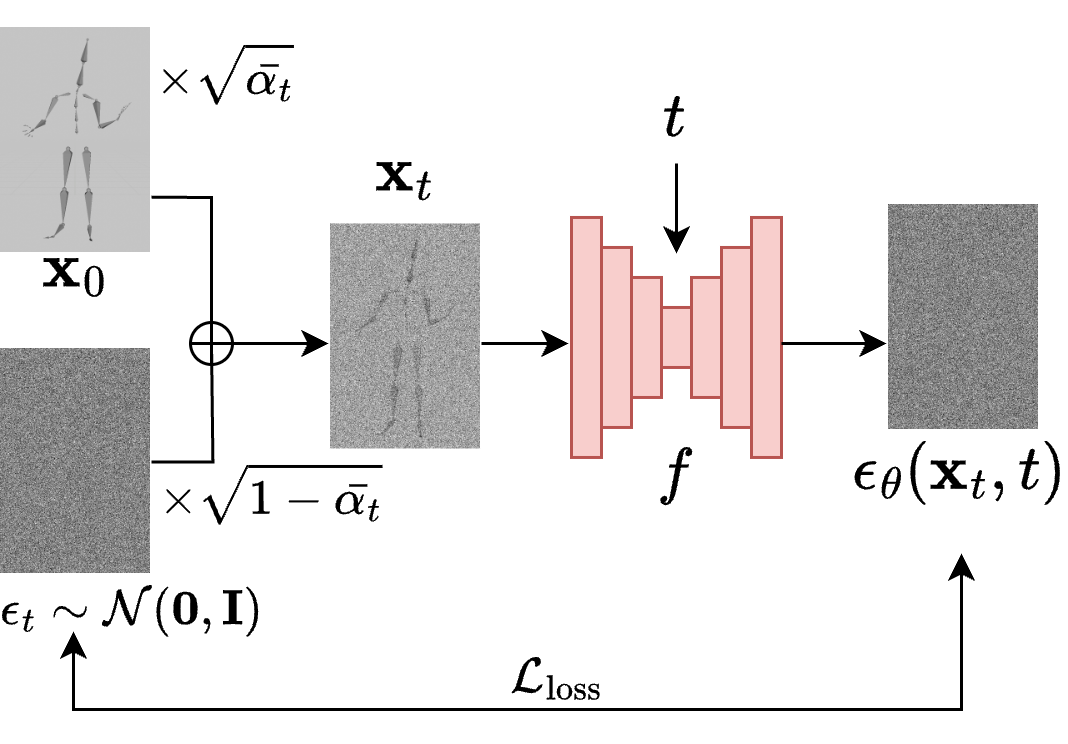
\includegraphics[width=\textwidth]{AlgorithmForwardDiffusion.png}
\end{column}


	
\begin{column}{0.5\textwidth}
	\footnotesize
	\begin{algorithm}[H]
		\caption{Training} \label{alg:training}
		\begin{algorithmic}[1]
			\footnotesize
			\Repeat
			\State $\bx_0 \sim q(\bx_0)$
			\State $t \sim \mathrm{Uniform}(\{1, \dotsc, T\})$
			\State $\bepsilon\sim\mathcal{N}(\bzero,\bI)$
			\State Take gradient descent step on
			\Statex $\qquad \grad_\theta \left\| \bepsilon - \bepsilon_\theta(\mathbf{x}_t, t) \right\|^2$
			\Until{converged}
		\end{algorithmic}
	\end{algorithm}
%		\Statex $\qquad \grad_\theta \left\| \bepsilon - \bepsilon_\theta(\sqrt{\bar\alpha_t} \bx_0 + \sqrt{1-\bar\alpha_t}\bepsilon, t) \right\|^2$

%{\footnotesize
%	\noindent\rule[0pt]{\textwidth}{0.4pt}
%	Training
%	\noindent\rule[0pt]{\textwidth}{0.4pt}
%	\begin{tabbing}
%		{\bf Given} $x^k$, $\lambda^{k-1}$, and parameter $\beta \in (0,1)$. \\*[\smallskipamount]
%		Let $\lambda := \lambda^{k-1}$. \\*[\smallskipamount]
%		{\bf Repeat} \\
%		\qquad \= 1.\ Let $z := \prox_{\lambda g}(x^{k} - \lambda \nabla f(x^{k}))$. \\
%		\> 2.\ {\bf break if} $f(z) \leq \hat{f}_{\lambda}(z, x^{k})$. \\
%		\> 3.\ Update $\lambda := \beta \lambda$. \\*[\smallskipamount]
%		{\bf Return} $\lambda^{k} := \lambda$, $x^{k+1}:=z$.
%\end{tabbing}}
%	\noindent\rule[10pt]{\textwidth}{0.4pt}
	
\end{column}

\end{columns}

\end{frame}

\begin{frame}{Reverse Diffusion Process}
	
\small
$p_{\theta}(\mathbf{x}_T) = \mathcal{N} (0, \mathbf{I}) \qquad 
p_{\theta}(\mathbf{x}_{t-1} | \mathbf{x}_t) = \mathcal{N}(\mathbf{x}_t; \mu_\theta(\mathbf{x}_t), \sigma_t^2 \mathbf{z})
$
%\begin{columns}
%	\begin{column}{0.5\textwidth}
%		
%	\end{column}
%	\begin{column}{0.5\textwidth}
%		
%	\end{column}
%\end{columns}

$\mu_\theta(\mathbf{x}_t) = 
\frac{1}{\sqrt{\alpha_{t}}} ( \mathbf{x}_t - 
\frac{1-\alpha_t}{ \sqrt{1 - \bar{\alpha_{t}} }}
\epsilon_{\theta} (\mathbf{x}_t,t))$
%\vspace{-20pt}
%\begin{figure*}

%	& \text{ ;where } \bar{\boldsymbol{\epsilon}}_{t-2} \text{ merges two Gaussians (*).} 

\begin{columns}
	\begin{column}{0.43\textwidth}
		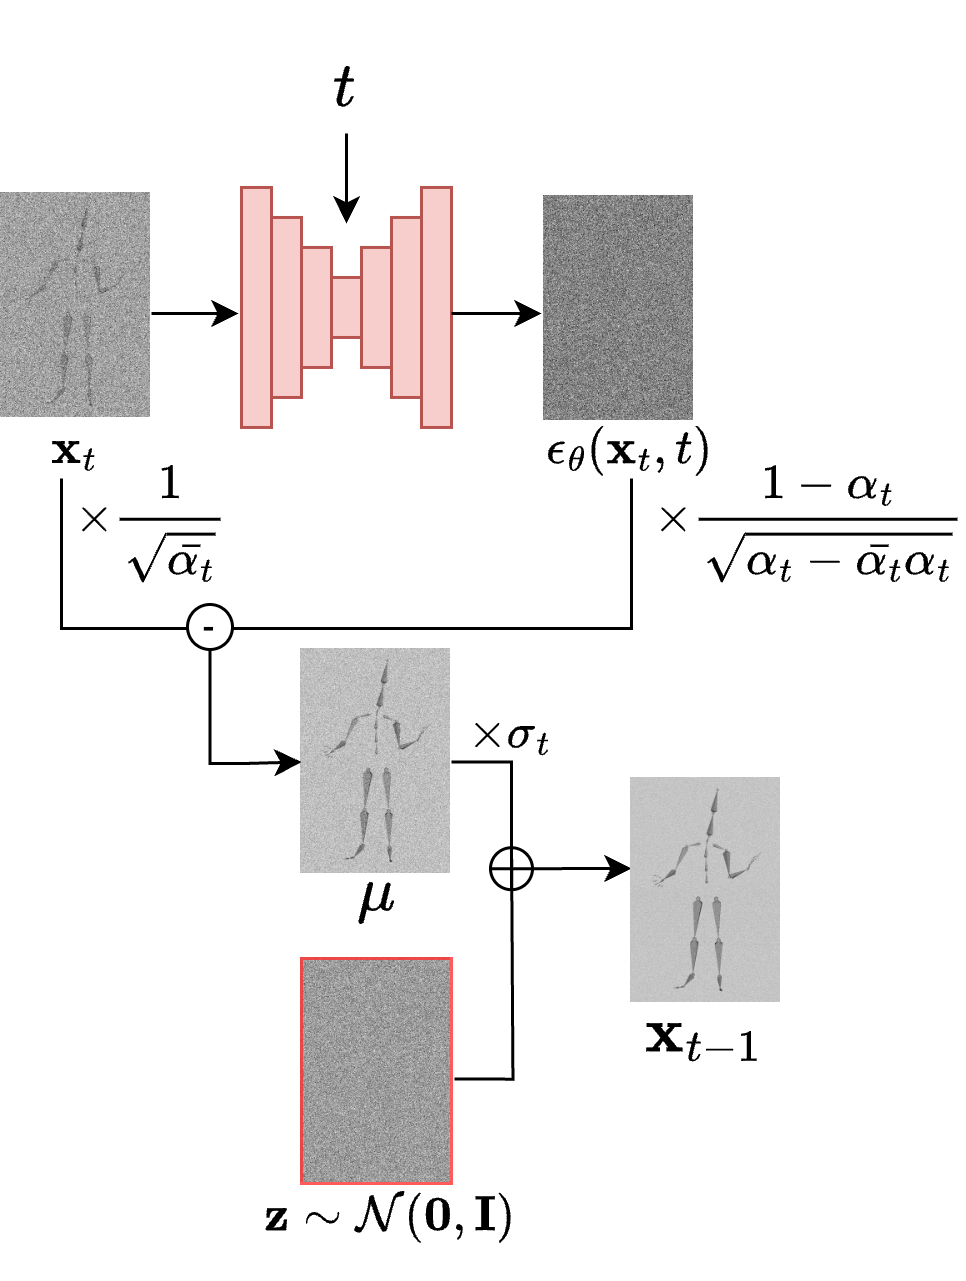
\includegraphics[width=\textwidth]{AlgorithmSamplingDiffusion.png}
	\end{column}
	
	\begin{column}{0.57\textwidth}
		\footnotesize
		\begin{algorithm}[H]
			\caption{Sampling} \label{alg:sampling}
			\footnotesize
			\begin{algorithmic}[1]
					\footnotesize
					\State $\bx_T \sim \mathcal{N}(\bzero, \bI)$
					\For{$t=T, \dotsc, 1$}
					\State $\bz \sim \mathcal{N}(\bzero, \bI)$ if $t > 1$, else $\bz = \bzero$
					\State $\mu = \frac{1}{\sqrt{\alpha_t}}\left( \bx_t - \frac{1-\alpha_t}{\sqrt{1-\bar\alpha_t}} \bepsilon_\theta(\bx_t, t) \right) $
					\State $\bx_{t-1} = \mu + \sigma_t \bz$
%					+ \sigma_t \bz
%_\theta (\mathbf{x}_t,	 t)
					\EndFor
					\State \textbf{return} $\bx_0$
					\vspace{.04in}
				\end{algorithmic}
		\end{algorithm}
\end{column}

\end{columns}

\end{frame}

%	\algrenewcommand\algorithmicindent{0.5em}
%	\begin{figure}[t]
	%		\begin{minipage}[t]{0.495\textwidth}
		%			\begin{algorithm}[H]
			%				\caption{Training} \label{alg:training}
			%				\small
			%				\begin{algorithmic}[1]
				%					\Repeat
				%					\State $\bx_0 \sim q(\bx_0)$
				%					\State $t \sim \mathrm{Uniform}(\{1, \dotsc, T\})$
				%					\State $\bepsilon\sim\mathcal{N}(\bzero,\bI)$
				%					\State Take gradient descent step on
				%				\Statex $\qquad \grad_\theta \left\| \bepsilon - \bepsilon_\theta(\sqrt{\bar\alpha_t} \bx_0 + \sqrt{1-\bar\alpha_t}\bepsilon, t) \right\|^2$
				%					\Until{converged}
				%				\end{algorithmic}
			%			\end{algorithm}
		%		\end{minipage}
	%		\begin{minipage}[t]{0.495\textwidth}
		%			
		%		\end{minipage}
	%		\vspace{-1em}
	%	\end{figure}

\begin{frame}{Hàm Loss $\mathcal{L}$}
		\textbf{Hàm loss}: $\mathcal{L} = \sum_{t=1}^{T} \mathcal{L}_t$
		
	\begin{itemize}
		\item Diffusion: $\mathcal{L}_{\text{loss}}= \mathbb{E}_{\mathbf{x}_0, \epsilon_t \sim N(0, I), t} \left[ \| \epsilon_t - \epsilon_\theta(\mathbf{x}_t, t) \|^2 \right]$
	\end{itemize}
	\begin{figure}
		\centering
		\includegraphics[width=\linewidth]{NoiseLoss}
	\end{figure}
\end{frame}


\begin{frame}{Đặc điểm của việc học dữ liệu Motion}
	
\begin{columns}
	\begin{column}{0.55\textwidth}
		\textbf{Quan hệ giữa dữ liệu cử chỉ và âm thanh}:
		\begin{itemize}
			\item Một đoạn cử có thể bao gồm nhiều âm thanh.
			\item Mỗi âm thanh có thể tương ứng với nhiều đoạn cử chỉ khác nhau.
		\end{itemize}
%		Baseline: \textbf{MDM}  (Human Motion Diffusion Model)
		\textbf{Khó khăn}
		\begin{itemize}
			\item Dữ liệu ít, chi phí cao
			\item Thiếu nhãn và dữ liệu tương ứng giữa âm thanh, cử chỉ.
			\item Quá trình sinh có thể dể điều khiển 
%			hơn GAN.
		\end{itemize}
		liệu
%		\textit{Mô hình Diffusion}:
%		\begin{itemize}
%			\item Ít yêu cầu về dữ liệu gắn nhãn
%			\item Khả năng tương tác và điều chỉnh dễ dàng
%			\item Tính ổn định cao
%		\end{itemize}
	\end{column}
	\begin{column}{0.45\textwidth}
		
		\begin{columns}
			\begin{column}{0.5\textwidth}
				\begin{figure}
					\includegraphics[width=\textwidth]{ProbabilityDensityFunctions.png}
					\caption{\scriptsize Phải chuẩn hoá (diện tích dưới đường cong phải tích phân thành một)}
				\end{figure}
			\end{column}
			\begin{column}{0.5\textwidth}
				\begin{figure}
					\includegraphics[width=\textwidth]{ScoreFunction.png}
					\caption{\scriptsize Không cần chuẩn hoá.}
				\end{figure}
			\end{column}
		\end{columns}
		
		
		
		\begin{columns}
			\begin{column}{0.5\textwidth}
				\centering
				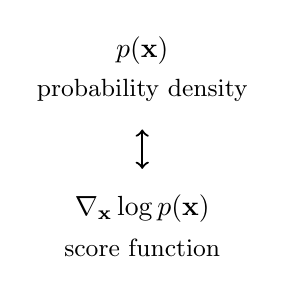
\begin{tikzpicture}
					\node at (0, 1) {$p(\mathbf{x})$};
					
					\node at (0, 0.5) {\small \text{probability density}};
					
					\draw[<->, thick] (0, 0) -- (0, -0.5);
					
					\node at (0, -1) {$\nabla_\mathbf{x} \log p(\mathbf{x})$};
					
					\node at (0, -1.5) {\small \text{score function}};
				\end{tikzpicture}
				
			\end{column}
			\begin{column}{0.5\textwidth}
				\begin{figure}
					\includegraphics[width=\textwidth]{CompareScoreFunction.png}
					\caption{\scriptsize score function vs probability density}
				\end{figure}
			\end{column}
		\end{columns}
	\end{column}
\end{columns}

\end{frame}
	
	
%	
%		if $L$ is not known (usually the case), can use the following line search:
%	\noindent\rule[-5pt]{\textwidth}{0.4pt}
%	
%	\noindent\rule[10pt]{\textwidth}{0.4pt}
%	
%	typical value of $\beta$ is $1/2$, and 
%	\[
%	\hat{f}_\lambda(x,y) = f(y) + \nabla f(y)^T (x - y) + 
%	(1/2\lambda)\|x - y\|_2^2
%	\]